\documentclass[12pt, twocolumn]{article}
\usepackage{amsmath}
\usepackage{amsfonts}
\usepackage{graphicx}
\usepackage{mathtools}
\usepackage{fullpage}
\usepackage{float}
\usepackage{color, soul}

\begin{document}
\title{ 6.867 Term Project: \\ An Exploration of Deep Learning and \\ Convolutional Neural Nets for Image Classification\\ }
 \author{Kathryn Evans, Andres Hasfura and Remy Mock}
\maketitle

\section{ Introduction} 
Artificial Neural networks (ANN) are a useful machine learning framework. Their primary benefit is that instead of specifying the basis functions relating input to output, they are learned.  This is especially useful for when the optimal basis function is complicated or non-intuitive, such as in the case of images.


Through this course, a simple singular layer artificial neural network was presented. However, much like the neural networks in the human brain visual system , the architectures used for machine learning neural networks can be more complex than a single hidden layer. The idea of utilizing many layers is known as deep learning.  Increasing layers, allows for more complex input/output relationships and an ability to classify based on both information from low and high level features.

Deep learning, although not a recent idea, has recently exploded in popularity due to rise in labeled data and general purpose GPU programming and is revolutionizing very important subfields within artificial intelligence. Machine learning, machine vision, and natural language processing are examples of areas in which the use of deep learning has produced large jumps in performance on difficult test sets. Deep nets are now being used anywhere from pedestrian detection for autonomous vehicles \cite{Szarvas2006}, to facial expression recognition \cite{Li2015} to classifying whether or not a selfie is good \cite{Karpathy}. 
	
Not only do deep nets contain more hidden layers but also a multitude of different types of layers. Each layer type has different connectivity and objective, allowing for a greater richness of information. In the case of images, convolutional layers are especially beneficial for examining spatially close pixels to determine features. Arrangements of convolutional layers as well as other types of layers leads to Convolutional Neural Networks (CNN). 

In this project, we want to explore the benefits of deep nets as well as convolutional neural networks for image classification.  Our first goal is implement our own multilayer neural networks and convolutional neural networks. From this we hope to gain insights on the benefit on image classification performance of firstly, additional fully connected hidden layers and secondly, more complicated layer types.  Not only do we want to gain familiarity with the concepts and tools used in deep learning but we hope to benchmark our home made software on MNIST. 

Our second goal is to attempt to replicate results from Yann LeCun on the classification of the MNIST data sets for more complicated frameworks like LeNet \cite{LeCun1998}. For this we will use a professional deep learning library to get faster results and be able to quickly build extensive architectures. 

Thirdly, we hope to do some analysis on the results of multilayer architectures. The generalities we hope to explore include the following: How does the number of layers affect the amount of training data needed?  How much variance is there in the output results due to random initialization/dropouts? How large of a dataset do we need to train on to be able to classify accurately?  To quickly cycle through a number of different tests we will utilize TensorFlow, a professional software by Google.

This paper is organized as follows. First we will introduce fully connected and convolutional neural networks with an emphasis on types of layers and implementation. We will also describe the dataset which we use for testing our implementations, MNIST, as well as those networks we wish to replicate.  Then we will describe our results for each of the three goals previously stated, starting with results from the implementation with software we built, then replication and lastly expanding to deeper analysis. 

\section{Methodology}
In this project, we seek to implement a version of multi-layer neural network for supervised learning on images. We plan on trying our implementation on the MNIST dataset, so that we do not have to worry about data generation and labeling. Because we are specifically interested in applying our implementation to images, we also hope to see benefit of making the network out of convolution layers, where not all nodes are connected and we will compare this to a implementation with fully connected layers.

 We will then compare our rudimentary approach to a professional library for deep learning, specifically the TensorFlow platform. Undoubtedly, the professional library will allow for better results and interesting conclusions. However, building and implementing a simplified version will give a better understanding into how the neural network works. 

\subsection{Division of Labor}
	
 
 For the project we split the work into three parts for each of the members. Kathryn Evans built and analyzed the CNN. Andres Hasfura led the implementation of TensorFlow and complex architectures for replication of results. Remy Mock built the fully connected multilayer neural nets. We worked collaboratively to do parameters searches and design experiments. 

\subsection{Neural Network Basics}

In general, the idea of a neural network is to replace specific basis functions with learned basis functions. The basis functions are learned from the input data in the first layer of learning, and then utilized by a second layer which learns the relationship of the output data from those selected features.

\begin{equation}
a_j^{(1)}= \sum_{i=1}^N w_{ji}^{(1)} x_i+w_{j0}^{(1)}
\end{equation}
\begin{equation}
z_j= g(a_j)
\end{equation}

Where $g(x)$ is a nonlinear map of input to $(0,1)$, generally tanh or sigmoid. The activation, $a_j$  depends on the data, $x_i, \; i=\{1,...N\}$, learned weights $w_{ji}^{(1)}$ and bias $w_0^{(1)}$. 

The second layer learns in a similar fashion and can be described for $K$ output classes and $M$ features in the hidden layer as
\begin{equation}
a_k^{(2)}= \sum_{j=1}^M w_{jk}^{(2)} z_j+w_{k0}^{(2)}
\end{equation}
\begin{equation}
f_k= \tilde{g}(a_k^{(2)})
\end{equation}
 
where $\tilde{g}(x)$ is the  another nonlinear map, not necessarily the same as $g(x)$ and $f_k$ is really our prediction $h_k(x,w)$. 

\begin{figure}
\includegraphics[scale=.6]{simpleNN.png}

\caption{Visualization of a simple Neural Network with 1 hidden layer \cite{Bishop} . }
\label{fig:basicNN}
\end{figure}






\subsubsection{Back-propagation}

To perform stochastic gradient descent on the neural net, the back-propagation algorithm is used. Back-propagation uses the errors calculated in the forward propagation to calculate activations to calculate the necessary gradients with respect to the cost function $J$. Stochastic gradient descent is then used to update the weights with the following equation, 
\begin{equation}
w^{(t+1)} = w^{(t)} + \eta_t \nabla_w J(w^{(t)})
\end{equation}

where $\eta$ is  the learning rate and the choice of that parameter varies as it is to be chosen to optimize results for each particular model on the data-set.

The error function $J(w)$ we will attempt to minimize is 
\begin{equation}
J(w)= l(w) + \sum_{i=1}^N\lambda_{i}(\|w_i\|_F^2);
\end{equation}

Where  $\lambda$ is a regularization term to prevent overfitting and $l(w)$ is the negative loglikelihood function,

\begin{equation}
\scriptsize
l(w)=\sum_{i=1}^N \sum_{k=1}^K [-y^i_k log(h_k(x_i,w))-(1-y^i_k)log(1-h_k(x_i,w))]
\end{equation}


\subsection{Multi-layer Neural Network}


For each fully connected layer the forward propagation is straight forward, as you simply  chain the formula for a single hidden layer together for more layers.  For backwards propagation, the error for each fully connected layer, $l$ is computed from the error of its output layer, $l+1$  

\begin{equation}
\delta^{(l)}=((W^{(l)})^T \delta^{(l+1)}) \cdot f ^{\prime} (z^{(l)})
\end{equation}

Which create the the following derivatives for weights and biases, 
\begin{equation}
\nabla_{W^{(l)}}J(W,b;x,y) = \delta^{(l+1)}(a^{(l)})^T
\end{equation}
\begin{equation}
\nabla_{b^{(l)}}J(W,b;x,y)= \delta^{(l+1)}
\end{equation}

the weights are then adjusted accordingly in the gradient descent.



\subsubsection{Implementation}
Using MATLAB, we have implemented the Multi-layer Neural Network. It is soft-coded so the hidden layers and number of hidden nodes per layer can easily be altered. The function created cells for the weights of each layers and initialized the weights randomly between -1 and 1.
\newline
A sigmoid function shown below is used as the activation function.

\begin{equation}
\tilde{g}(x)= g(x) = \frac{1}{ 1+e^{-x}}
\end{equation}

A stochastic gradient descent approach was used with a step size $\eta$ shown below.
\begin{equation}
\eta = \frac{ \alpha}{ (\textrm{epoch} + \beta)^\gamma}
\end{equation}

where $\beta \leq 100$, $\gamma >.5$ and epoch is the number of times the descent method has gone through the training set.  
\newline\newline



\subsection{General Architecture of a Convolutional Neural Network}
As opposed to a fully connected neural network, a convolutional neural network is specifically designed to take advantage of the 2-D structure of an input image by considering only local connections. It also takes advantage of tied weights which reduced number of decision parameters, as well as pooling which results in translation invariant features. All these advantages, make CNN generally easier to train. 



\subsubsection{Convolutional Layer}
In a CNN, filters are learned to be used to identify key characteristics of a certain classification. These filters are convolved over subspaces of the original image dictated by the filter size, that learn features of these small segments of the larger image.  This transforms the 2-D images into a 3-D space.

 For a  $M * N $ size image, using $K$ filters that are $m * n$,  after convolution, there are  $ K * (M - m + 1) * (N - n + 1) $ sub images. Using this method, we decrease the size of each image, but at the same time learn low level features. This is described for each image, $x_n$ for $n=1..N$ and for each filter $k=1...K$ in the convolution layer, $c$ as
\begin{equation}
a_{n,k}^{(c)}= x_n \ast w_k^{(c)} + b_k^{(c)}
\end{equation}
\begin{equation}
f_{n,k}= \tilde{g}(a_{n,k}^{(c)})
\end{equation}
 
 Where $\ast$ is the convolution operator. 
 
 The number of filters directly controls capacity and is chosen based on the number of available examples and the complexity of the task. The challenge is then to identify the correct filter size in order to obtain reasonable granularity of features, given a particular dataset.

Also CNNs introduce the idea of tied weights, which mean that certain connections affiliated with a particular filter between one layer to the next are defined to be the same. The use of tied weights dramatically reduces the number of parameters needed to define network compared to a fully connected network of similar size. This idea is shown in Fig. \ref{fig:conv}.



\begin{figure}
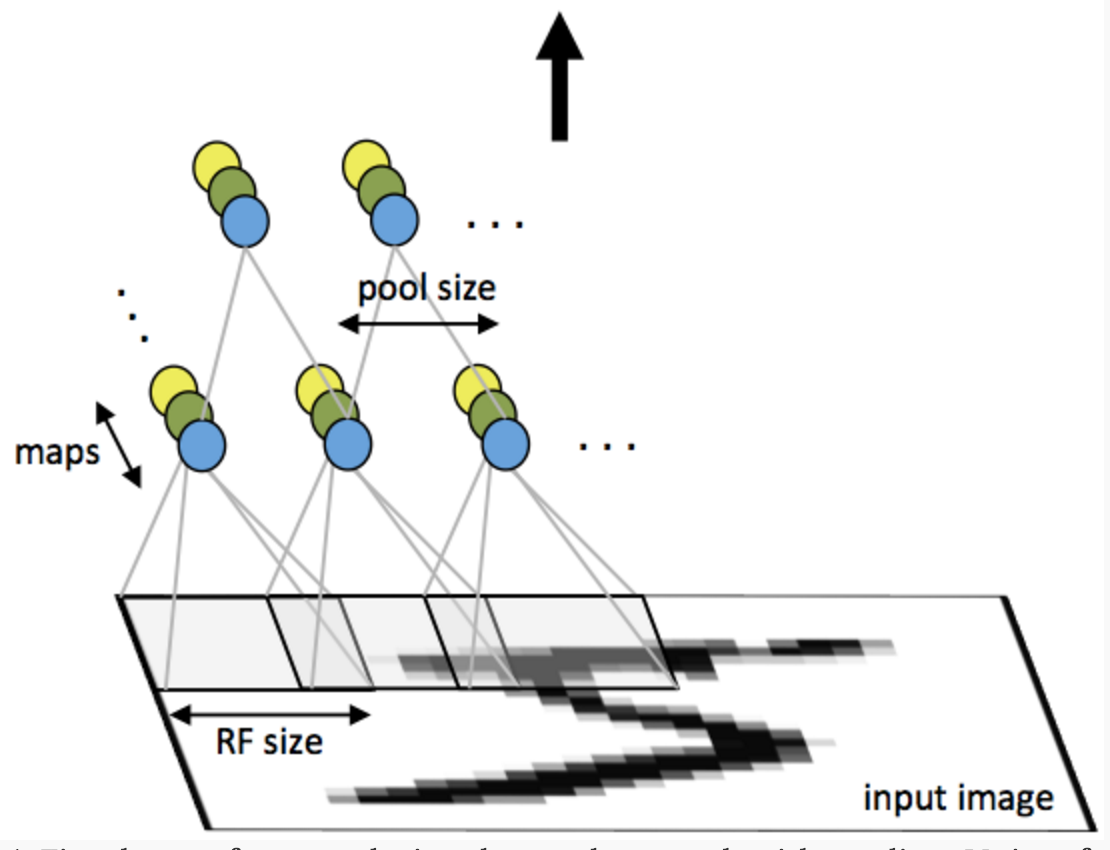
\includegraphics[scale=.4]{convgraphic.png}

\caption{Layer of a convolutional neural network with pooling. Nodes of the same color have tied weights and units of different color represent different filter maps \cite{StanfordTut}. }
\label{fig:conv}
\end{figure}


\subsubsection{Pooling Layer}
The features learned using convolution are next used for classification. Previously with the fully connected neural network we utilized a softmax classifier, but this can be computationally challenging and expensive. Instead, pooling layers take advantage of a single parameter of these features, such as the mean, ( 'mean pooling') or max ( 'max pooling'), at  various regions in the image. Not only does this reduce the dimensionality of the result but can also help reduce over-fitting, a problem that is of serious concern for networks with increasing numbers of hidden nodes. 

The region to be pooled over is determined by the pooling dimensions. It again involves a convolution, this time between regions specified by the pooling dimensions and the results from the previous convolution layer. 

\subsubsection{Dropout}

Another common trick used in CNNs is the inclusion of drop-out layers which help to decrease the likelihood of over-fitting. It achieves this by essentially thinning out the number of hidden nodes by randomly dropping units during training.  A depiction of this effect is shown in Fig.~\ref{fig:dropout}. However, during test time all nodes are present. 
\begin{figure}
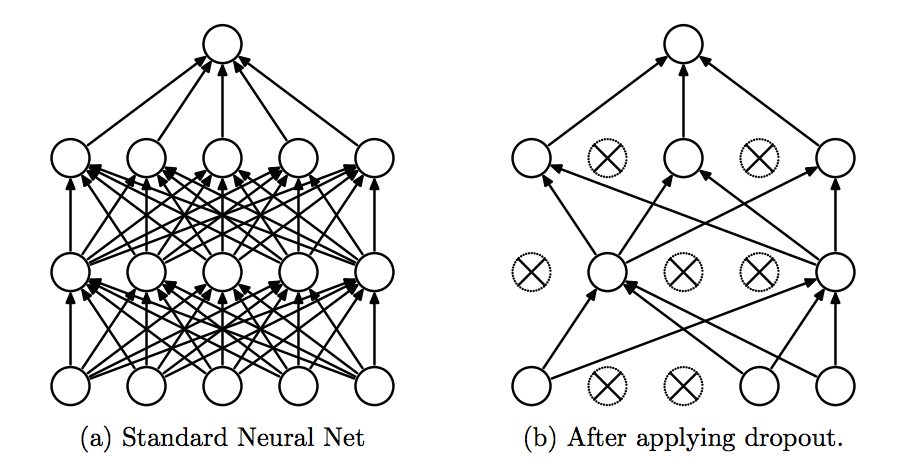
\includegraphics[scale=.52]{dropout.png}

\caption{Effect of dropout on a previously fully connected neural network. Dropped nodes are depicted as crossed out \cite{Dropout}. }
\label{fig:dropout}
\end{figure}

The simplest way to implement drop-out is to keep each node with probability, $p$, and otherwise discard it. The key benefit is that dropout is able to outperform regularization in neural networks for reducing over-fitting \cite{Dropout}. Dropout also has the added benefit of being able to evaluate exponentially many different neural network architectures depending on which nodes are dropped.
 
\subsubsection{Re-LU}

As we already mentioned, a major flaw of deep nets is that they can be computationally expensive. One of the main tools to minimize this is a smart selection of the activation function, $g$. 

Specifically using a rectified linear unit, (Re-LU) as opposed to more traditional sigmoids or tanh, can be beneficial in increasing the efficiency of a neural network \cite{imagenet}. The Re-LU function is simple, 

\begin{equation}
g(x)= \textrm{max}(0,x)
\end{equation}

This function is not smooth but because the computation of $g$ is simply a comparison, it is generally much faster than smooth approximates. It also allows for sparse activation of the neural network, eliminating nodes with negative activations. 

\subsubsection{Backprop for CNN}
For fully connected layers  the derivative calculation remains the same. However,  error propagations are more complicated through the pooling and convolutional layers. 

For the pooling layer, the error must be up-sampled to propagate backwards
\begin{equation}
\delta^{(l)}_k=\textrm{upsample}((W^{(l)}_k)^T \delta^{(l+1)}_k) \cdot f^{\prime}(z^{(l)}_k)
\end{equation}


For mean pooling, with pool dimension, $p$, this is equivalent to 
\begin{equation}
\delta^{(l)}= \frac{1}{p^2}  \textrm{kron}(\delta^{(l+1)}, \textrm{ones}(p))
\end{equation}
where kron, is the Kroneckor Tensor Product.

Thus for the convolution layer, the derivatives can be calculated as follows.
\begin{equation}
\nabla_{W^{(l)}}J(W,b;x,y) = \sum_{i=1}^m (a^{(l)}_i) \ast  \delta^{(l+1)}_k
\end{equation}
\begin{equation}
\nabla_{b^{(l)}}J(W,b;x,y)= \sum_{a,b}(\delta^{(l+1)}_k)_{a,b}
\end{equation}


\subsection{Professional Libraries}

Since deep learning has become increasingly popular, so too are optimized professional libraries  that allow students, researchers and hobbyists to easily build complex deep nets. . There are many of these libraries, but we chose to adopt TensorFlow, the open source software from Google \cite{TensorFlowGH}. We especially like TensorFlow because it is python based, has abundant tutorials, and is easy and intuitive to use. In addition, is uses an interface with Cuda for GPU processing to speed up results for image computations. \cite{TensorFlowWeb}. 



\subsection{Benchmarking with MNIST}


The MNIST is a well-known dataset of handwritten digits, 0-9, comprising 60,000 training examples and 10,000 test examples \cite{MNIST}  that can be used for image classification.  This data set arose from the U.S. Postal Service zip code database in order to help the scanning and transport of package to the right area. The images are all centered in 28 x 28.

\begin{figure}
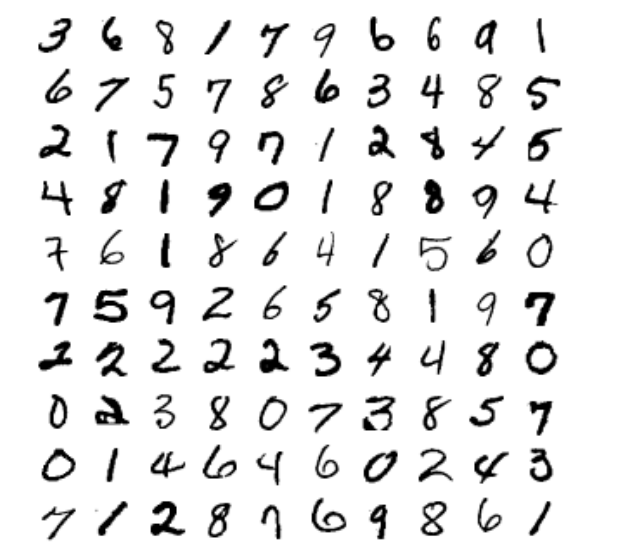
\includegraphics[scale=.8]{MNISTnos.png}
\label{fig:MNISTex}
\caption{Sample entries of the MNIST dataset \cite{LeCun1998}}
\end{figure}

Since the data-set has already been thoroughly explored  by many people including Yann LeCun \cite{LeCun1998}, it is a good data set on which to measure our success.  Replication of the architecture of both the fully-connected and convolutional multi-layer neural nets, (LeNet) provided in this paper is the one of the objective of our study. 

\subsubsection{LeNets}
The LeNet framework was developed by LeCun beginning in the 1980's. They provide a few examples of more complex CNN architecture on which we will compare our performance. 
The CNN LeNet-1 architecture consists of 5 layers, which are denoted by C1, S2, C3, S4, and F5.  The output of the first layer serves as
input to the next layer. C1 and C3 are convolution layers, and S2 and S4 are sub-sampling layers and the fifth layer is fully connected. \cite{LeCun89}

The CNN LeNet-4 architecture consists of 6 layers, which adds to LeNet-1 an additional hidden layer that is fully connected to its  input and output layers  \cite{LeCun95}.

LeNet-5 architecture expands on this even further by adding an additional layer, with gaussian connections. More details on the architecture chosen, including filter size number and pooling dimension are shown in Fig. ~\ref{fig:LeNet5}

 \begin{figure*}
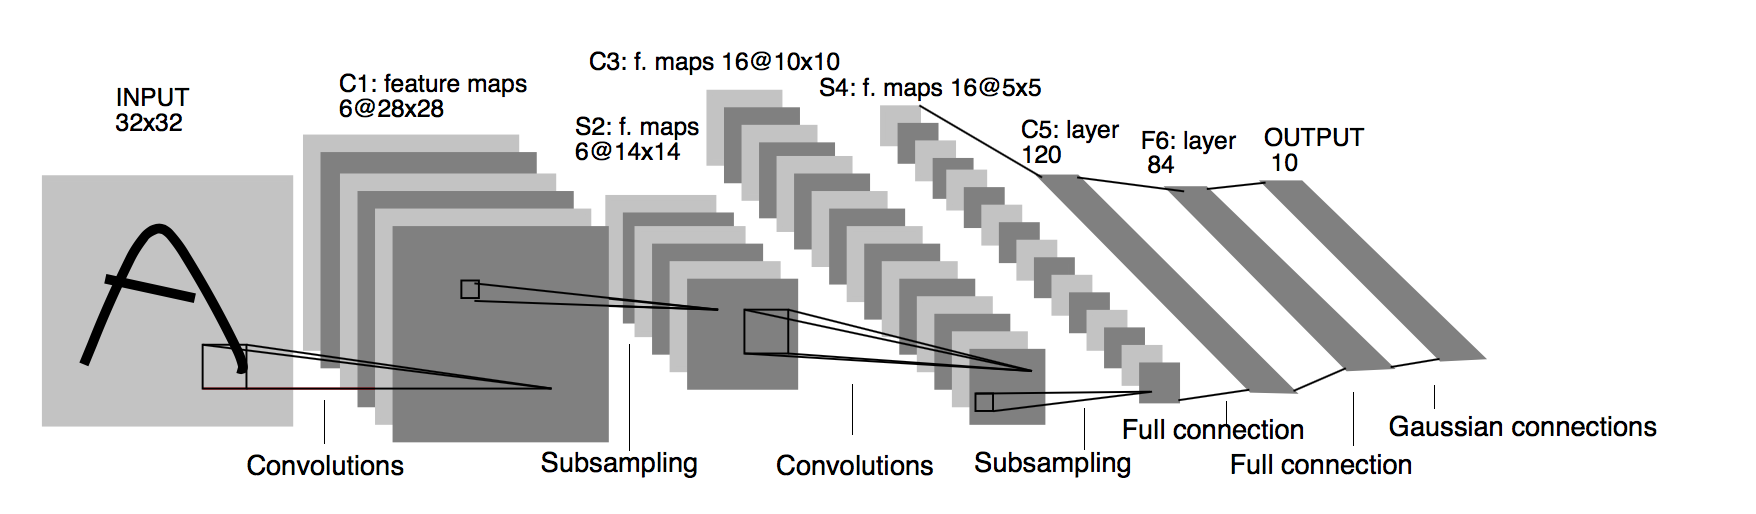
\includegraphics[scale=.6]{LeNet5.png}
\caption{Architecture for LeNet5 \cite{LeCun1998}}
\label{fig:LeNet5}
\end{figure*}



\section{Results}
We start by benchmarking our handmade mulitlayer and convolutional network on the MNIST dataset, and provide discussion about some of the challenges and difficulties behind building these deep nets. We then replicate the remaining deeper architectures presented by LeCun, but for these we use TensorFlow. We did not have access to GPU clusters, so we found it necessary to use TensorFlow's more computationally efficient implementations. Finally, we provide further analysis of the deep architectures, further illuminating characteristics of deep neural networks. 

\subsection{Multilayer NN}
The initial goal was to alter the two-layer neural network done for homework 3 to have the functionality to soft-code the number of hidden layers and the number of nodes per hidden layers.

Once this was done, a grid search was done to find the optimal parameters. Due to the fact that all results documented by others have been on the three-layer model (using two hidden layers), we decided to focus on the three-layer model. The parameters optimized include the number of hidden nodes and regularization $\lambda_1$ ,$\lambda_2$ and $\lambda_3$ for layers 1, 2 and 3 respectively.

For the architecture with 300 hidden nodes and 100 hidden nodes, we obtained the best testing accuracy of 6.2\% when $\lambda_1$ ,$\lambda_2$ and $\lambda_3$ were $10^{-3}$, $10^{-8}$ and $10^{-5}$. The testing error was extremely sensitive to  the regularization parameters, and even changing one of the parameters slightly increased the testing error significantly. 

\subsection{Simple CNN}
We began by building the most basic form of a convolutional neural network, which starts with a convolution layer, followed by one pooling layer, and finished with a fully connected layer to the output. This net was then trained and tested on the MNIST dataset to ensure proper implementation and extract performance and computation time metrics. 

As we discovered with neural nets, the devil is in the details. It is very difficult to find the optimal parameters for CNNs because of the high dimensional optimization space and the lack of generalization between architectures. Finding optimal parameters for a particular net says very little about the best parameters for another architecture. The space is too high dimensional for grid search and also highly non-convex, eliminating any guarantees for gradient descent based methods. 

After much research and trail-and-error, we converged on a set of parameters which achieved 2.7$\%$ on the MNIST dataset. The optimal combination for our architecture was 20 filters, 9 x 9 convolution kernels, and 2 x 2 pooling dimensions. We were only able to reach 2.7 error after the third epoch, after only one pass through the training data the net still produced 4.6$\%$ error. 

\subsection{Replication of NNs and LeNets Results}

We attempted to replicate the published results for testing error on MNIST for the network structures specified in LeCun's paper, \cite{LeCun1998}. Specifically we designed

\begin{itemize}
\item{2 layer fully connected with 1000 hidden nodes}
\item{3 layer fully connected with 300 then 100 hidden nodes}
\item{3 layer fully connected with 500, then 150 hidden nodes}
\item{5 layer convolutional network (based on LeNet-1)}
\item{6 layer convolutional network (based on LeNet-4)}
\item{7 layer convolutional network (based on LeNet-5)}
\end{itemize}

\begin{table*}
\begin{center}
\begin{tabular} { |c | c | c | }
    \hline
    NN Type & LeCun Error  &   Tensor Flow Error \\ \hline
    2-layer NN, 1000 hidden units & 4.5  & 5.8\\ \hline
    3-layer NN, 300+100 hidden units & 3.05  & 8.2 \\ \hline
    3-layer NN, 500+150 hidden units & 2.95  & 5.6\\ \hline
    5 layer CNN  (LeNet-1) & 1.7  & 3.1\\ \hline 
    6 layerCNN (LeNet-4) & 1.1 & 1.6\\ \hline 
    7 layer CNN (LeNet-5) &  0.95  & 2.3\\ \hline
  \end{tabular}
\caption{Comparison of Test Error results for multilayer ANN and CNN with published results \cite{LeCun1998}.}
\label{table:MNISTLeCun}
\end{center}
\end{table*}




Although the LeNets come with specified filter numbers, sizes, and pooling sizes, there remained many parameters that were not given which make it non-trivial to replicate. These parameters included number of iterations, learning rates, batch size, dropout, pooling method, weight initializations, and others, all of which are not included clearly in the published results. Because results are so sensitive to the entire combination of parameters, knowing the few provided was not sufficient to reproducing his results. Therefore, we maintained the same network architecture, but did not restrict ourselves to only using the parameters specified in LeCun's paper. Instead, we were able to closely replicate the results using our own combination of the system's parameters.

Our 5 layer CNN, which was modeled after LeCun's LeNet1, is constructed as follows. Input images are fed through two convolution and pooling layer combinations in series, and finish with a fully connected layer. To implement our 6 layer CNN, modeled after LeCun's LeNet4, we simply added another fully connected layer to the tail, and similarly appended another fully connected layer to LeNet4 for our 7 layer LeNet5 emulation. 

In general we fixed certain parameters to make our search simpler. For any convolutional layer we fixed filter size to be 5x5 pixels and pooling size to be 2x2 pixels. We found that the first convolution worked well with with 32 filters and second with 64.   We left all fully connected layers with 1024 nodes. 

Also we understand that LeCun cites convergence in testing error after 10-12 times the number of training data in iterations for LeNet-5 \cite{LeCun1998}. However, since it takes greater than 4 minutes to run each of the multilayer CNNs for 1 epoch and we were more interested in experimenting with a variety of different parameters, we capped the iterations at 100,000. Obviously these will not be as successful as runs that were carried out for an order of magnitude more iterations and therefore we do not expect to match Lecun's results perfectly.  Our best results are shown in Table ~\ref{table:MNISTLeCun}. 

\begin{table*}
	\begin{center}
		\begin{tabular} { |c | c | c | }
			\hline
			NN Type & Mean error &   Variance\\ \hline
			2-layer NN, 1000 hidden units & 6.8  & 0.63\\ \hline
			3-layer NN, 300+100 hidden units & 11.4  & 3.9 \\ \hline
			3-layer NN, 500+150 hidden units & 8.9  & 3.4\\ \hline
			5 layer CNN  (LeNet-1) & 3.8  & 1.07 \\ \hline 
			6 layerCNN (LeNet-4) & 3.7 & 1.01\\ \hline 
			7 layer CNN (LeNet-5) &  3.9  &1.3\\ \hline
		\end{tabular}		
		\caption{Comparison of Mean Accuracy and Variance results for multilayer ANN and CNN}
		\label{table:variance}
	\end{center}
\end{table*}

\subsection{Variance of Results}
In Table ~\ref{table:MNISTLeCun}, we include only the maximum performance on the test data. However, this may not be a great metric since we found with our results, that when the data-set on the exact same network with exactly the same parameters with the randomized initial weight, we get a shockingly large range of testing errors. This is due to the weight initialization and drop outs that happen in a random manner. We ran each of the nets list twenty times  to achieve the following results Table ~\ref{table:variance}. 

We reran two specific networks, the 2 layer fully connected and the 6 layer CNN, an additional 30 times and made histograms of the results so that the scatter could be visualized as well. These can be seen in Fig. ~\ref{fig:hist2layer} and Fig.~\ref{fig:histletnet4} respectively. 





The results show that the is low variance in the 2-layer fully connected neural network but high variance in both of the 3 layer fully connected networks. High variance could be indicative that many more iterations through the training data would be needed to converge to steady state weights and therefore a consistent test error. It could also be a sign that the cost space for that particular network is riddled with more local optima.  


\begin{figure}
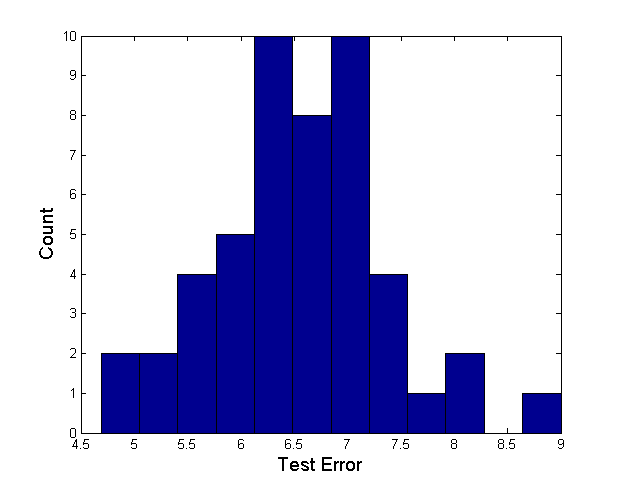
\includegraphics[scale=.5]{hist2layer.png}
\caption{Histogram for Test Error for the 2 layer 1000 hidden node network}
\label{fig:hist2layer}
\end{figure}

\begin{figure}
	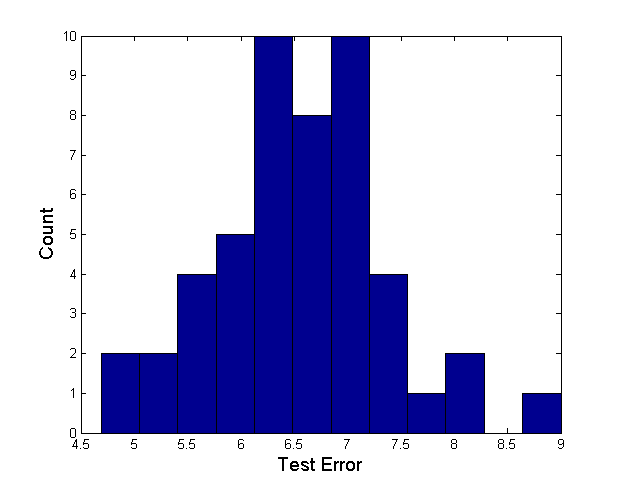
\includegraphics[scale=.5]{hist2layer.png}
	\caption{Histogram for Test Error for the LeNet network}
	\label{fig:histlenet}
\end{figure}




\subsection{Effect of Training Data Size}
One of the other main areas we wanted to investigate was how the relationship between amount of training data affects and testing error, changes for increasingly large networks. We decided to investigate this by running the 5 and 7 layer CNNs with the same parameters and iterations and gradually increase the percentage of the MNIST data we give as an input. These results are shown in Fig. \ref{fig:trainsize}.  

With the same number of iterations but fewer examples, a simple way to guess the size of dataset needed comes from mathematics.  We need at least the same number of equation and variables to solve a multi-variable equation. Since the number of unknown weights can be calculated(see appendix), we expect the number of training data needed $T$ is proportional to this number. We expect that the network does a increasingly better job at classifying until it hits $T$ and plateaus after this number.

\begin{figure}
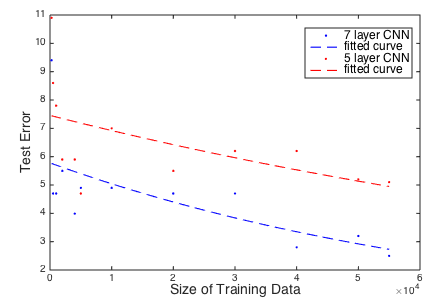
\includegraphics[scale=.5]{trainingsize.png}
\caption{Effect of Training Data Size for 5 and 7 layer CNN}
\label{fig:trainsize}
\end{figure}


In these plotted figures we see that as expected the networks ability to classify correctly increases as it is given more dat-sets to train on. However the learning curve was not as steep as expected. Even with only 256 data-sets the network was able to perform with only a 10.4\% test error.

\subsection{Comparison to a two-layer model}
According to the Universal Approximation theorem, in a compact and continuous data-set the two-layer neural network can perform as well as any multi-layer neural network given enough hidden nodes. We decided to see if this theory can be applied to our data-set by varying the number of hidden nodes and measuring the test error on a two layer model.
 
 \begin{figure}
 	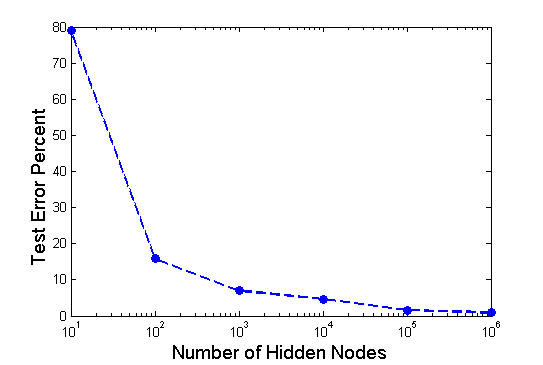
\includegraphics[scale=.6]{errorvshiddennodes.png}
 	\caption{Effect of number of hidden nodes on a two layer model}
 	\label{fig:numhidden}
 \end{figure}
Looking at the figure 8, it is evident that the networks performs better with increasing the amount of hidden nodes. However training takes increasingly longer since the network is linearly proportional to the number of hidden parameters which is proportionally to the number of hidden nodes (see appendix). Furthermore once the number of parameters is on the order of the number of data-sets we may see no additional benefit of increasing the number of nodes. This is due to the same reason discussed in the section before regarding the solving a multi-variable equation.

\section{Conclusions}
We implemented the multi-layer neural network and convolutional neural network and optimized them for varying parameters. The best test errors obtained on the networks we implemented were 6.2\% and 2.7\% for the multi-layer network and convolutional network respectively. We then replicated these networks using TensorFlow, compared our results with Lecun's results and did some further analysis to gain deeper insight.
 Using TensorFlow, we obtained our best result with a test error of merely 1.6\% using the network architecture that corresponds with LeNet-4. Considering that our best results were from deep networks and not from two-layer model, it is evident to us that deep neural networks are superior to the simple two-layer model. Deep neural networks are a powerful tool and it is no surprise that deep learning is increasing in popularity.

\bibliographystyle{unsrt}
\bibliography{references}
\section{Appendix}
\subsection{Calculation of the number of Parameters}
 Calculating the number of parameters of the two layer network with 1000 hidden nodes, 
\begin{equation*}
\textrm{params} = 784*1000 + 1000* 10 = 794000
\end{equation*}

and in the case of the three layer model with 300 and 100 hidden nodes,
\begin{equation*}
\textrm{params} = 784*300 + 300*100 + 100* 10 = 266200
\end{equation*}
It is evident that the three-layer network outperforms the two-layer network with less parameters. 

<<<<<<< HEAD
In regards to time complexity, it is evident that the bottleneck of the function is back-propagation. Since the complexity back-propagation is related to the number of parameters it is also evident that the three-layer method has a lower time complexity.

It is clear from the two factors above that multi-layer is more efficient and is no surprise that deep learning is increasing in popularity.


\section{Conclusions}
We implemented the multi-layer neural network and convolutional neural network and optimized them for varying parameters. The best test errors obtained on the networks we implemented were 6.2\% and 2.7\% for the multi-layer network and convolutional network respectively. We then replicated these networks using TensorFlow, compared our results with Lecun's results and did some further analysis to gain deeper insight.
 Using TensorFlow, we obtained our best result with a test error of merely 1.6\% using the network architecture that corresponds with LeNet-4. Considering that our best results were from deep networks and not from two-layer model, it is evident to us that deep neural networks are superior to the simple two-layer model. Deep neural networks are a powerful tool and it is no surprise that deep learning is increasing in popularity.

\bibliographystyle{unsrt}
\bibliography{references}
=======
In regards to time complexity, it is evident that the bottleneck of the function is back-propagation. 
>>>>>>> c257ad97f7d245e04b712fad6a1076f37418a4be
\end{document}
